\section{Experimentation \& Results}\label{results}

This section describes scenarios that are represent unique features enabled by
the DRE in Cyclus. As such, they are based on a general scenario that may be
modeled by many, likely most, available fuel cycle simulators. A simple UOX-MOX
binary recycle system is chosen in order to reduce the complexity of the fuel
cycle and highlight departures from available simulators. A simulation timeframe
of 50 years is chosen, sufficient to display all relevant effects. The nominal
parameters of all common facilities in the simulation are shown in Appendix
\ref{}. Importantly, reactors are allowed to be fueled by either UOX or MOX,
with a preference for MOX over UOX.

In order to involve dynamicism in the simulation, the population reactors grows
linearly over time at a rate of 1 reactor every 5 years with an initial
population of 20 reactors. Further, the presence of the the recycled-fuel supply
chain appears at some time, $t_{sc}$, after the beginning of the simulation,
chosen to be 10 years into the simulation. Therefore, all reactors will be
neccessarily fueled with UOX before $t_{sc}$ and MOX as available thereafter. 

The diagram of the base-case fuel cycle is shown in Figure \ref{fig:base}. It
represents a simple light-water reactor recycle scenario, with repository flows
comprised of separated minor actinides. The remaining portion of this section
perturbs this basic fuel cycle.

\begin{figure}
  \begin{center}
    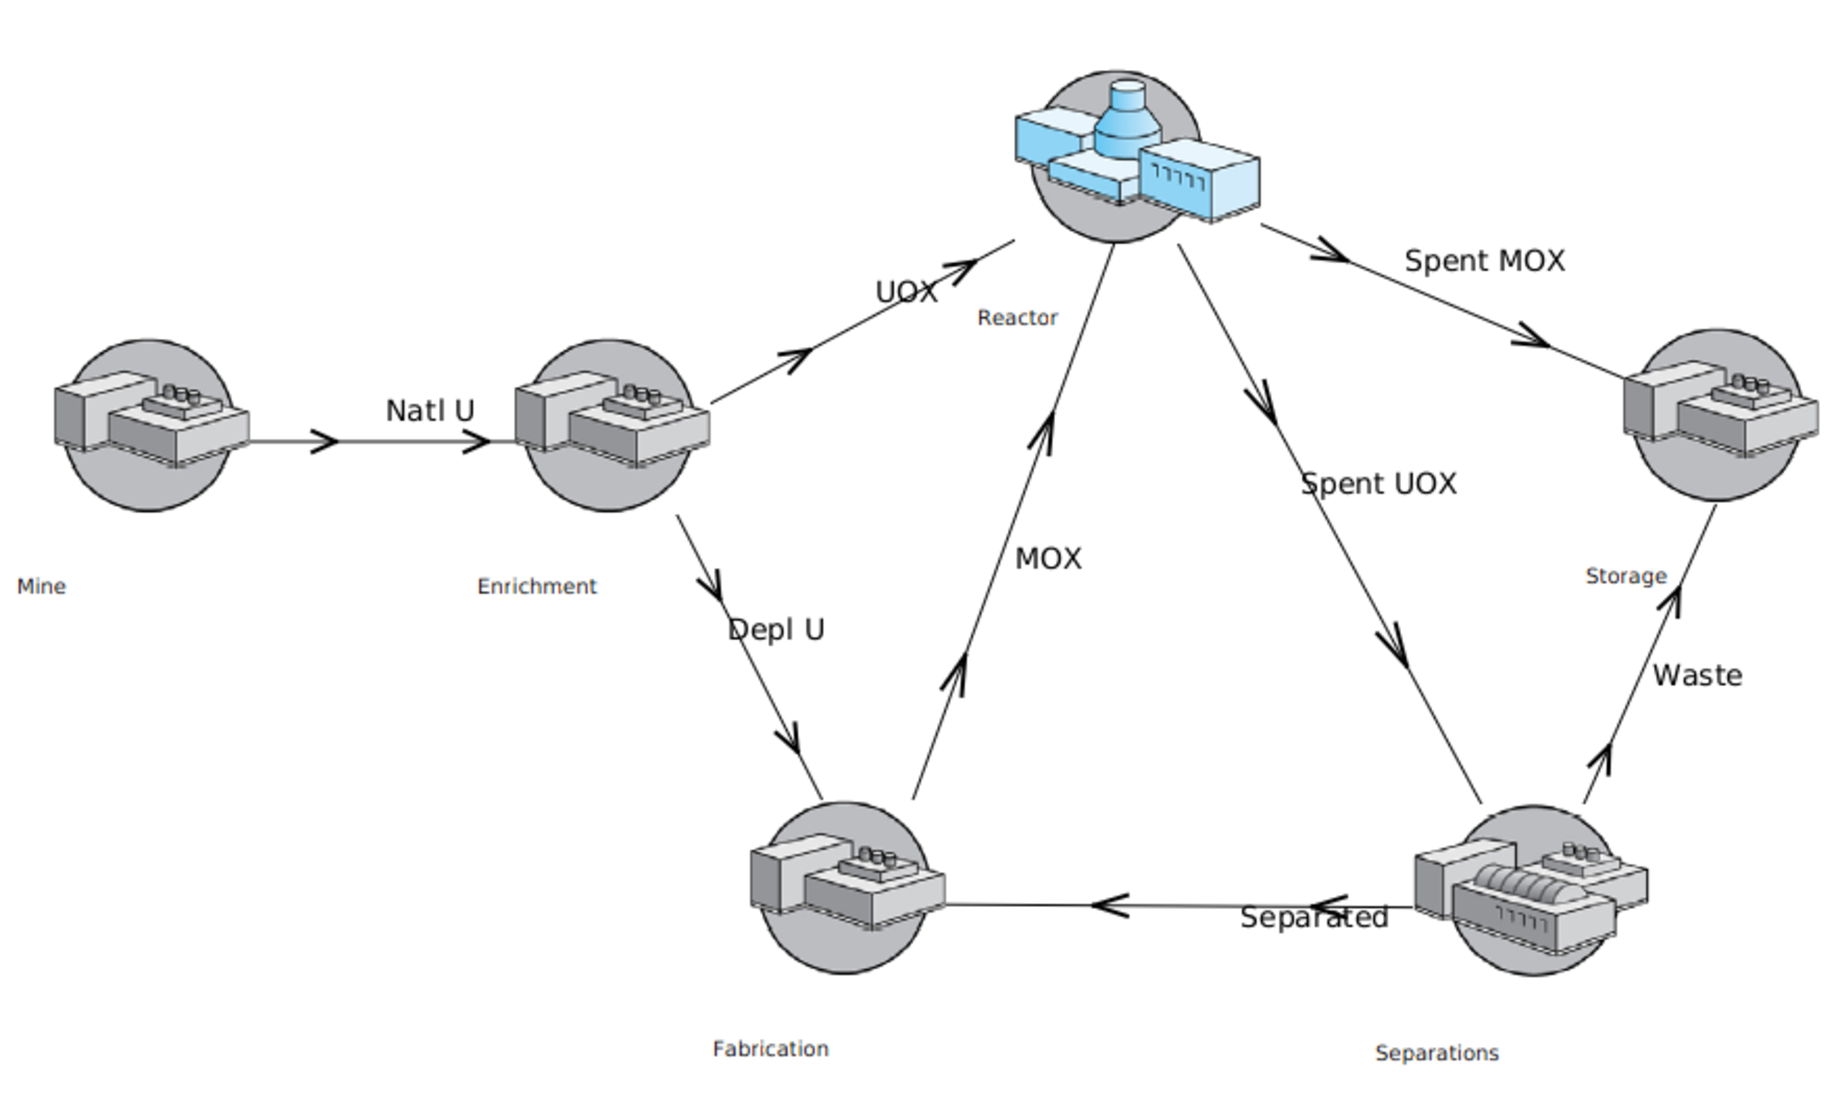
\includegraphics[height=10cm]{base.pdf}
    \caption[]{
      \label{fig:base}
      The base, single-pass MOX fuel cycle used for all comparisons.}
  \end{center}
\end{figure}

\subsection{Fuel Cycles with Demand Fungibility and Supply Disruption}

The DRE provides a unifying framework in which any instance of supply and demand
can be formulated and solved. This flexibility lends itself well to dynamic
simulation in which the state of actors in a simulation, by definition, can (and
will) change as the simulation progresses. In order to show case the types of
simulations that are enabled by this feature, a fuel cycle simulation is
constructed that has multiple types of reactor fuel input and a defined supply
disruption within the recycled-fuel supply chain.

To motivate this type of scenario, consider a nation state with a MOX and
UOX-based reactor fuel supply chain in addition to a (possibly former) weapons
program. Two sources of light-water reactor fuel exist for the entirety of the
simulation: UOX fuel and civilian MOX. At some time, $t_0$, MOX from
military-grade plutonium becomes available at production rate of $p_{MOX,
  m}$. Such a scenario is not outside of the realm of possibility; the United
States, for instance, is currently building the Mixed Oxide Fuel Fabrication
Facility for just such a purpose. Further, consider the following preference
distribution: civilian MOX is preferred over military MOX which is preferred
over civilian UOX. Preferring civilian MOX is reasonable because of the
likelihood of existing fuel contracts and a desire of reaching a reactor cycle
equilibrium. Preferring military MOX over civilian UOX is reasonable due to a
desire to reduce the stockpile of weapons-grade plutonium and increasing overall
resource utilization. Of course, a fuel cycle analyst is free to explore the
results due to different preference distribution choices.

Given sufficient supply of civilian MOX, such a scenario would not fully utilize
the source of military-based MOX. However, the supply of civilian MOX depends on
the entire recycled-fuel supply chain. Utilizing Cycamore and Cycamore-like
entities, this supply chain is comprised of a \texttt{Separations} facility
archetype and a \texttt{FuelFab} facility archetype. For use in this
proof-of-concept simulation, the Cycamore \texttt{Separations} archetype was
forked and updated to include a ``pausing'' feature. That is, it can be
temporarily removed from the simulation for some time, simulating a disruption
or disturbance. Due to the flexibility of the DRE, one expects the
military-based MOX to be fully utilized during the supply disruption.

% description of military source and pause

% deployment description

\begin{figure}
  \begin{center}
    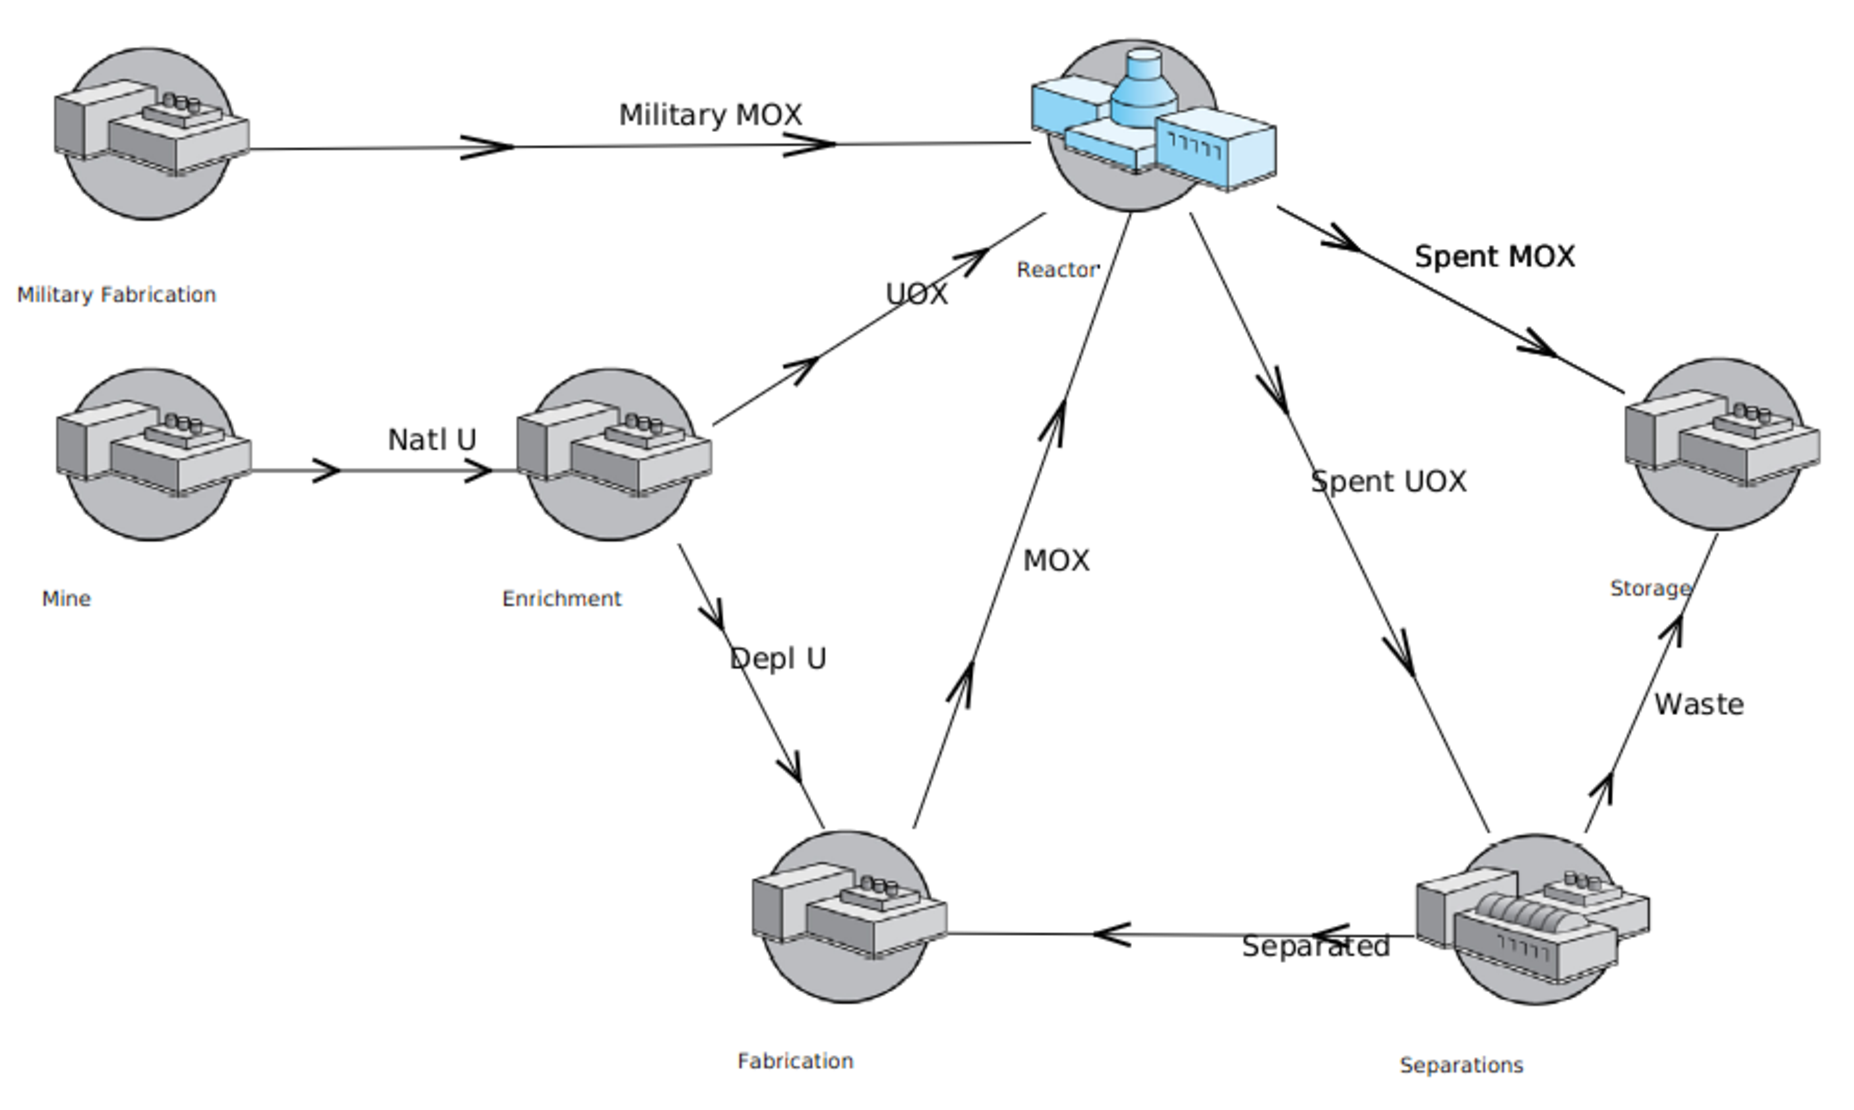
\includegraphics[height=10cm]{military.pdf}
    \caption[]{
      \label{fig:military}
      The base fuel cycle shown in Figure \ref{fig:base} with the addition of a
      military-based MOX fuel source.}
  \end{center}
\end{figure}

% with/without pause results

% timing between greedy/coin


\subsection{Fuel Cycles with International Instruments}

The DRE also allows for different geographical and managing entity
representations to be laid over otherwise regional-agnostic fuel cycles and
affect the outcome of possible trades within those fuel cycles. To showcase this
feature, consider the following two-region simulation. In one region, say Region
A, a fuel cycle with both UOX and MOX-based fuels is available. Further, this
region has an over-abundance of supply of fuel and can thus provide fuel
services to other regions. A second region, Region B, houses a simple,
once-through fuel cycle. This fuel cycle setup is shown in Figure
\ref{fig:region}.

\begin{figure}
  \begin{center}
    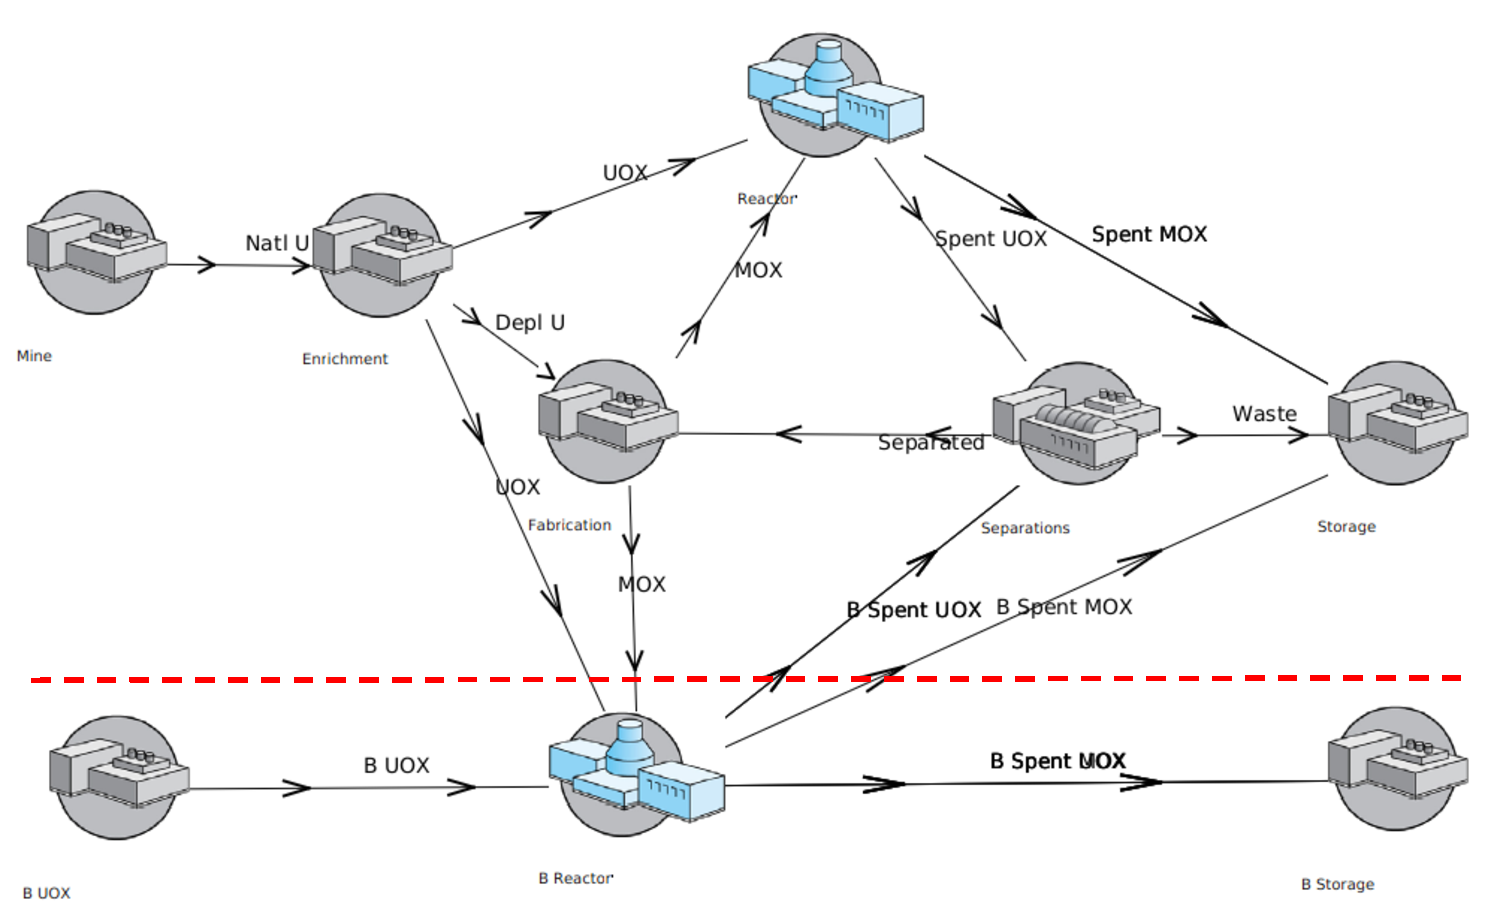
\includegraphics[height=10cm]{region.pdf}
    \caption[]{
      \label{fig:region}
      A two-region set of fuel cycles separated by a dotted-red line. The upper
      region (Region A) includes a one-pass MOX fuel cycle, and the bottom
      region (Region B) includes a once-through fuel cycle connected to the
      one-pass MOX fuel cycle.}
  \end{center}
\end{figure}

In an undeturbed setting, preferences can be set such that fuel input into
Region B is always preferred over domestic fuel production. In other words, a
preference distribution for fuel supplied to Region B could have the following
relation

\begin{equation}\label{eqn:bigdefault}
  p_{MOX, a} > p_{UOX, a} > p_{UOX, b} > 1.
\end{equation}

\noindent
This preference distribution implies that Region B's domestic fuel cycle will
never be utilized -- it will always be fueled by Region A, as long as Region A
has available capacity. However, a tariff can be applied which perturbs
preference values along arcs connecting Region A fuel suppliers with Region B
fuel consumers. Consider a tariff defined by function in Equation
\ref{eqn:tariff} with preferences adhering to the relation provided in Equation
\ref{eqn:bigp1}, which guarantees a strict preference ordering under $f(t)$.

\begin{equation}\label{eqn:tariff}
f(t)
\begin{cases}
1, & \text{if } t < t_0 \\
\frac{p_{UOX, b} - 1}{p_{UOX, a}}, & \text{if } t_0 \leq t < t_1 \\
\frac{p_{UOX, b} - 1}{p_{MOX, a}}, & \text{if } t_1 \leq t < t_2
\end{cases} 
\end{equation}

\begin{equation}\label{eqn:bigp1}
  p_{UOX, b} \left( 1 - \frac{p_{UOX, a}}{p_{MOX, a}} \right) > 1.
\end{equation}

Choosing nominal values that satisfy Equations \ref{eqn:bigdefault} and
\ref{eqn:bigp1}, e.g., $p_{MOX, a} = 9$, $p_{UOX, a} = 4$, and $p_{UOX, b} = 2$,
one arrives at actual preference values as shown in Figure \ref{fig:prefs}.

\begin{figure}
  \begin{center}
    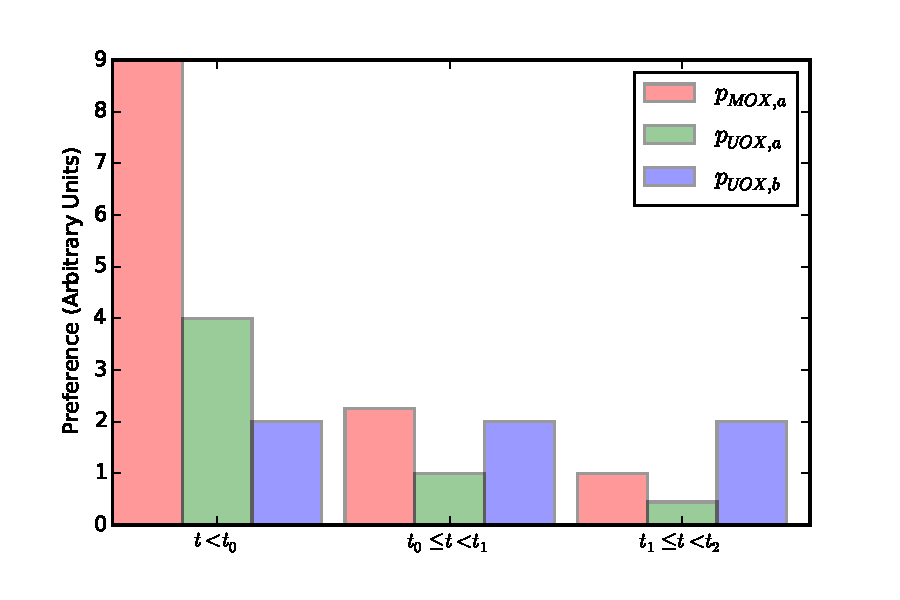
\includegraphics[height=7.5cm]{tariff_prefs.pdf}
    \caption[]{
      \label{fig:prefs}
      Resulting preference values for incoming fuel commodities in Region B
      after tariffs have been applied.}
  \end{center}
\end{figure}


% deployment description

% fc diagram

% with/without tariff results

% timing between greedy/coin
